Das Balancing, wie im Kapitel \ref{tGl_Balancing} erklärt, ist eine wichtige Funktion damit der Akku nicht zerstört wird. Das Ganze soll möglichst einfach aufgebaut und mit dem Mikrocontroller ansteuerbar sein. Wie in Abbildung \ref{fig:Balancing} ersichtlich, wurde dies mit einer P-Kanal MOSFET-Schaltung ermöglicht. Der Widerstand am Drain des P-Kanal-MOSFET reguliert den Strom mit dem die einzelnen Zellen ausgeglichen werden. Damit die Schaltung mit einem Mikrocontroller gesteuert werden kann, braucht es einen N-Kanal-MOSFET, der das Gate des P-Kanal MOSFET auf Ground zieht. Mit dieser einfachen Schaltung ist es möglich, die sechs Zellen des Akku zu balancen.

\begin{figure} [H]
	\centering
	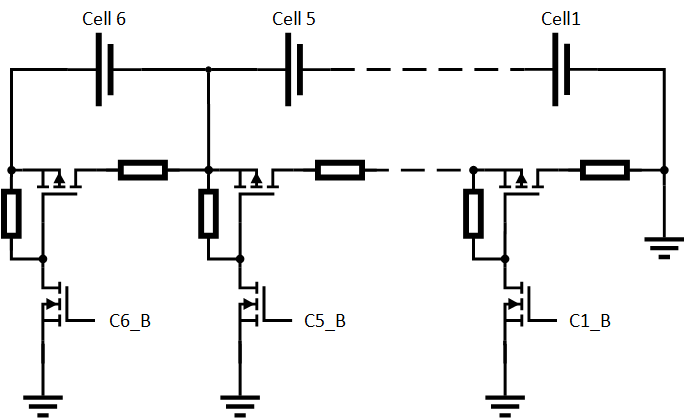
\includegraphics[width=0.6\linewidth]{images/Balancing}
	\caption{Balancing}
	\label{fig:Balancing}
\end{figure}


